\documentclass[12pt,a4paper,openany]{scrbook}

\include{Allgemein/packages}
\include{Allgemein/commands}

\usepackage{biblatex} %Imports biblatex package
\usepackage{float}

\addbibresource{bib/literature.bib}



%------------------------------------Links-----------------------------------------------------------------------%
\newcommand{\linkPi}{https://www.reichelt.de/raspberry-pi-3-b-4x-1-4-ghz-1-gb-ram-wlan-bt-raspberry-pi-3b--p217696.html}

\newcommand{\linkPiNT}{https://www.reichelt.de/raspberry-pi-netzteil-5-v-2-5-a-micro-usb-schwarz-nt-musb-25-sw-p167078.html}

\newcommand{\linkMstick}{https://eckstein-shop.de/M5StackM5StickCPLUSESP32-PICOMiniIoTDevelopmentKit2CInfrared2FRTC2FMic2FLED2FIMU2FPMU}

\newcommand{\linkBuzzer}{https://www.reichelt.de/sg/de/entwicklerboards-aktives-piezo-buzzer-modul-debo-piezo-p239111.html}


\begin{document}
	
	\include{Kapitel/titlepage} 
	\newpage
\chapter*{Hardwarebeschreibung Raspberry Pi}

\section{Einleitung: Vorstellung Raspberry Pi}
Der Raspberry Pi ist ein opensource Minicomputer, welcher ursprünglich als kostengünstiges System für Lernzwecke im Bereich der Programmierung gedacht war. [1]  \\
Besonders in der Makerszene erfreut sich der Raspberry Pi einer großen Beliebtheit. Es sind Projekte vom Desktopcomputer [1] bis hin zur Steuerung und Überwachung heimischer 3D-Drucker [3] realisierbar.\\ 
%Das Produktprotfolio reicht vom leistungsschwächeren Raspberry Pi (1Ghz singlecore, 512 MB RAM) zum leistungsstärkeren Raspberry Pi 
\\[3mm]


	\begin{figure}[!h]
	\centering
	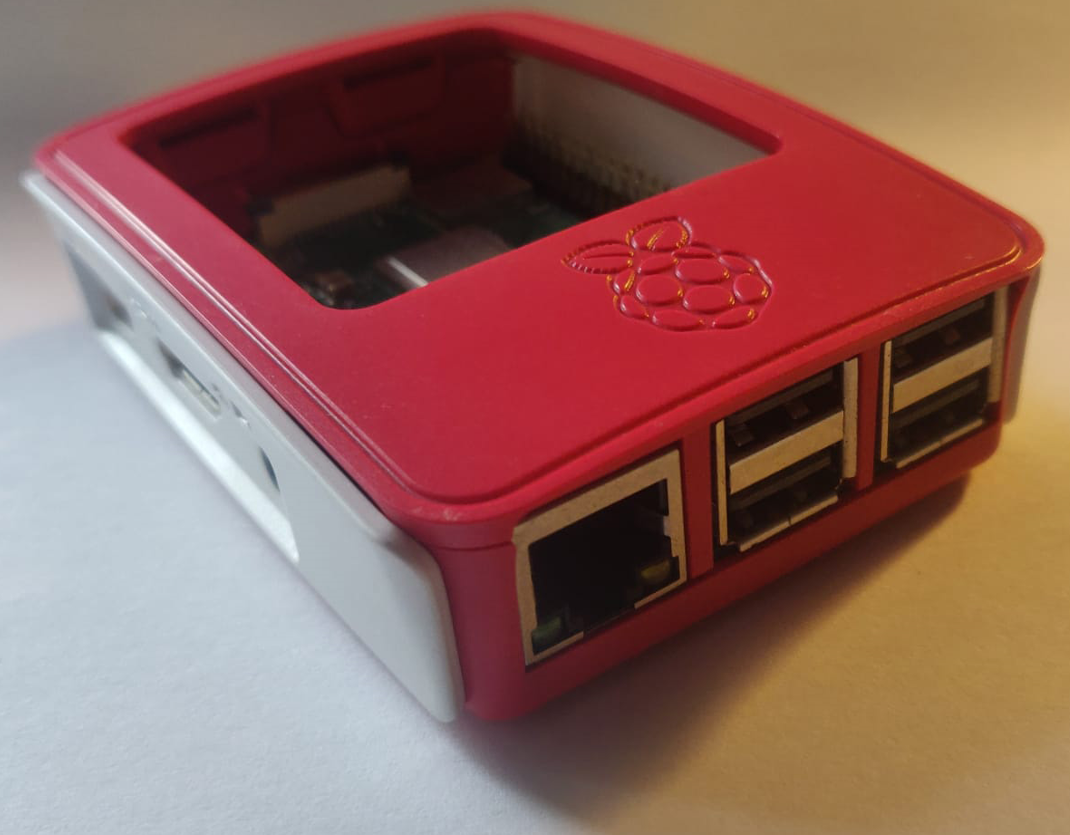
\includegraphics[height=250pt]{img/pi_mitgehaeuse.png}
	\caption{Raspberry Pi 3B+ (eigenes Foto)}
	\label{Bildlabel}
\end{figure}	


\chapter{Raspberry Pi für das Projekt}
Für das Projekt Überwachungssystem mittels der IMU des M5 Sticks soll ein\\ 
Raspberry Pi 3B+ als sogenannter IoT Broker und als Aktor für den Alarm genutzt werden.\\
%Das Modell 3B+ verfügt über eine Rechenleistung von
Der Raspberry Pi 3B+ wurde für das Projekt am Geeignetsten eingestuft. Er verfügt über einen Gigabit-LAN Anschluss welcher mit Hilfe eines Ethernetkabels für eine stabile Verbindung mit dem Rooter des Heimnetzwerkes sorgen soll. Verglichen mit älteren Raspberry Pi Modellen ist der 3B+ mit einer etwas stärkeren CPU, sowie einer WLAN und Bluetooth Karte ausgestattet, welche die Möglichkeiten bieten das Projekt um mehr IoT Geräte, sprich Sensoren und Aktoren zu erweitern. Zudem ist der preisliche Unterschied (Unverbindliche Preisempfehlung) zu den Vorgängermodellen marginal.  

	\begin{figure}[!h]
	\centering
	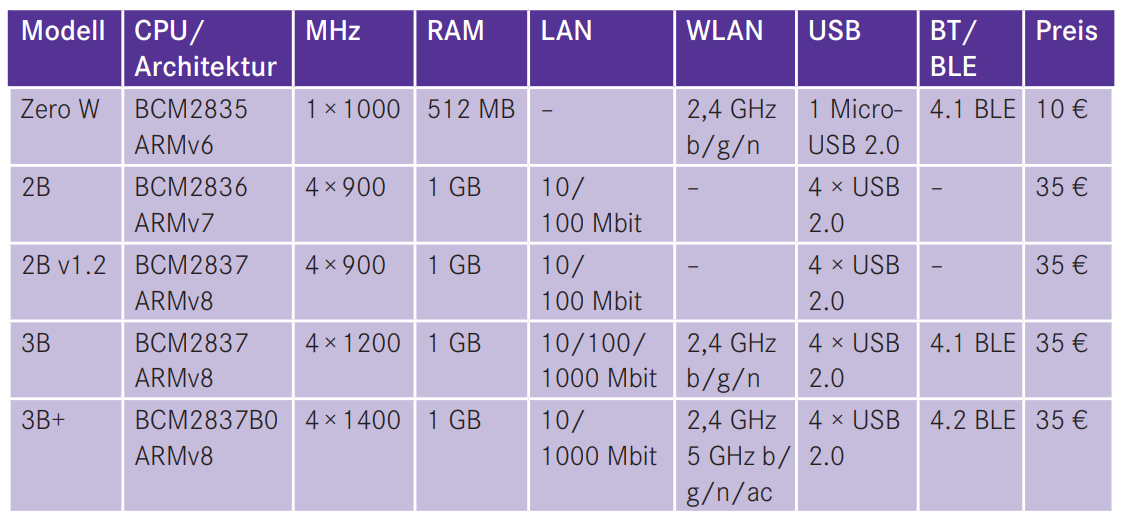
\includegraphics[height=200pt]{img/tabelle_pi_vergleich}
	\caption{Vergleich der verschiedenen Raspberry Pi Modelle (Buch Huewe IoT S. 59)}
	\label{Bildlabel}
\end{figure}


\section{Anschlussmöglichkeiten Anhand Raspberry Pi 3B+}
Der Raspberry Pi 3B+ verfügt im Allgemeinen über folgende Anschlussmöglichkeiten:\\[3mm] 
$\bullet$ HDMI   \\ %\hspace{20pt} $\bullet$ 
$\bullet$ 3,5mm AUX\\ 
$\bullet$ 4 $\times$ USB 2.0 \\ 
$\bullet$ Ethernet 1Gbit/RJ45\\ 
$\bullet$ CCI (Camera Connector Interface)\\ 
$\bullet$  DSI (Display Serial Interface)\\
$\bullet$ 40 GPIO-Pins\\
$\bullet$ Steckplatz für die microSD-Karte\\
$\bullet$ Micro-USB Anschluss für die Stromversorgung des PIs\\
Quelle: IOT at Home S.60\\ [10mm]

	\begin{figure}[!h]
		\centering
		
\includegraphics[height=250pt]{img/platzhalter}
		\caption{Hardwarebezeichnung auf Pi mit Beschriftung}
		\label{Bildlabel}
	\end{figure}
Für das Projekt sind insbesondere die GPIO-Pins und der Ethernetport von Bedeutung.\\

  

\section{Weitere Hardware im Bezug auf den Raspberry Pi}
\subsection{Piezo Buzzer Modul}
	Um beim Auslösen der Alarmanlage ein Warnsignal zu erzeugen, soll ein aktives Piezo Buzzer Modul ST1143 der Marke Iduino eingesetzt werden.\\ Die Pins des Buzzers werden wie folgt mittels Jumperkabeln mit den GPIO Pins des Pis verbunden: [4, draeger]
	
	\begin{table}[!h]
		\centering
		\begin{tabular}{|p{5cm}|p{5cm}|} 
			\hline
			Buzzer & Raspberry Pi  \\ 
			\hline
			SIG (S)   & GPIO 4 \hspace{0,1cm}(Pin 7)\\  
			\hline
			VCC~ (+; mittlerer Pin)   & 3,3V 	\hspace{0,7cm}(Pin 1)         \\ 
			\hline
			GND (-)    & Ground  	\hspace{0,2cm}(Pin 6)         \\
			\hline
		\end{tabular}
	\caption{Verbindung ST1143 mit Pi}
	\end{table} 

	
	\begin{figure}[!h]
	\centering
	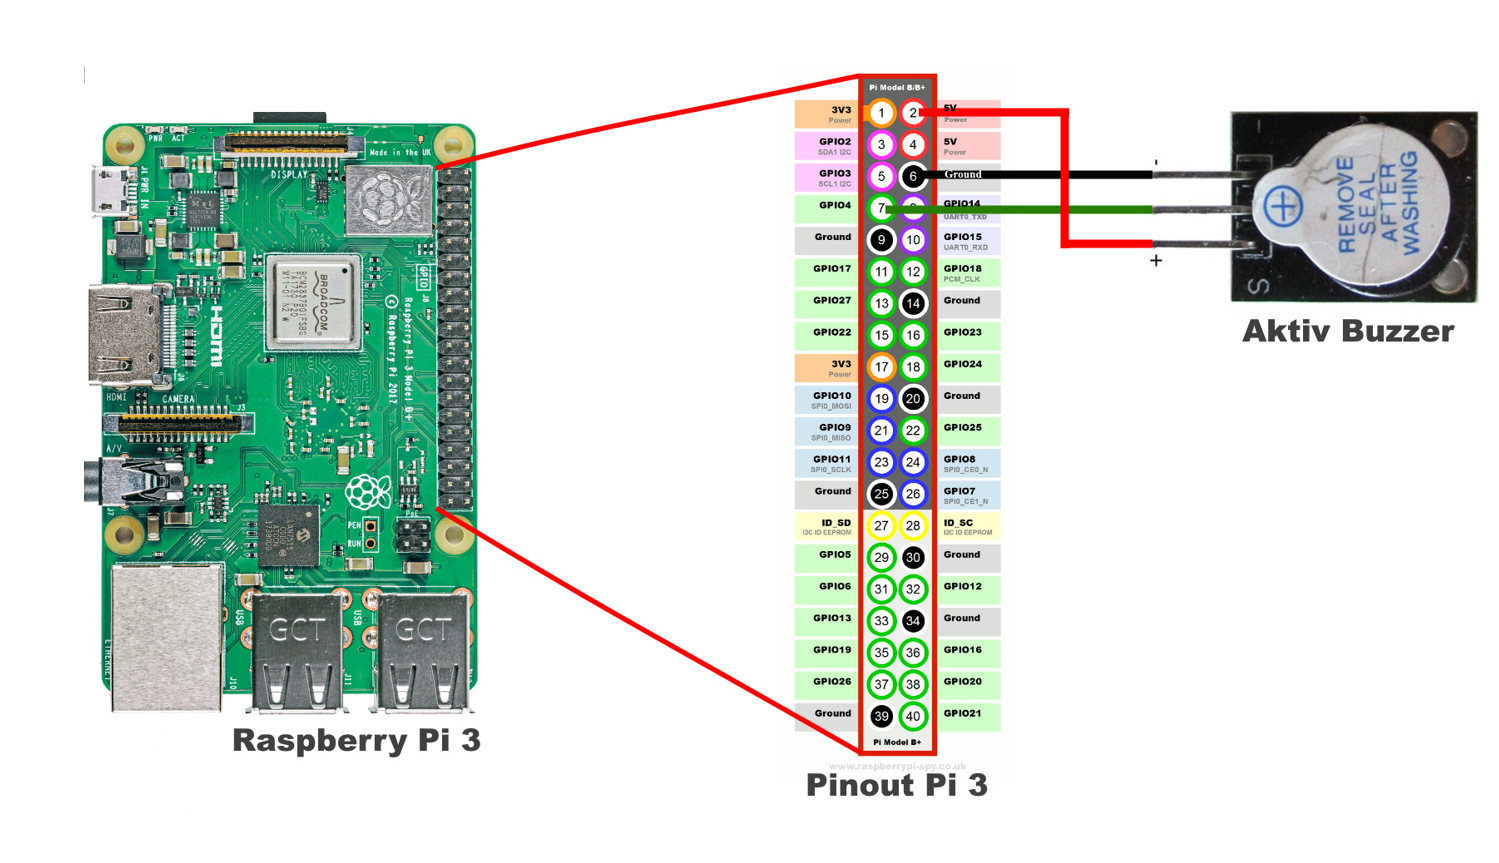
\includegraphics[height=300pt]{img/schaltplan}
	\caption{Schaltplan ST1143 an Raspberry Pi}
	\label{Bildlabel}
	
\end{figure}

	\begin{figure}[H]
	\centering
	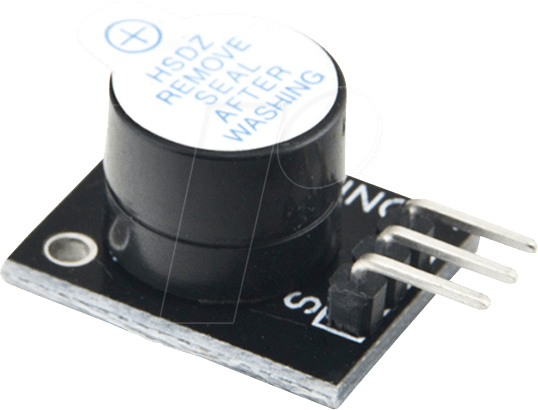
\includegraphics[height=150pt]{img/ST1143}
	\caption{Aktiver Piezo Buzzer ST1143 (Reichelt bestelllink)}
	\label{Bildlabel}
	\end{figure}



\subsection{Taster}

Der Alarm soll über zwei Tastermodule Iduino SE043 deaktiviert beziehungsweise manuell aktiviert werden können.\\ 
Die Module werden mittels Jumperkabeln mit den GPIO Pins des Pis verbunden. \\ 

	\begin{figure}[H]
	\centering
	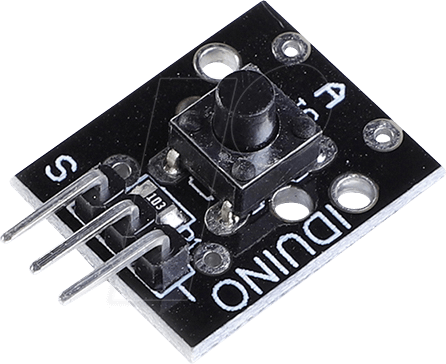
\includegraphics[height=150pt]{img/SE043}
	\caption{Iduino SE043 (Reichelt Bestelllink)}
	\label{Bildlabel}
\end{figure}

\begin{table}[H]
	\centering
	\begin{tabular}{|p{5cm}|p{5cm}|} 
		\hline
		Taster 1 (Aktivieren) & Raspberry Pi  \\ 
		\hline
		SIG(S)                   & GPIO 17 (Pin 11)               \\ 
		\hline
		VCC~(+, mittlerer Pin)                  & 5V (Pin 2)            \\ 
		\hline
		GND(-)                   & Ground (Pin 14)           \\
		\hline
	\end{tabular}
	\caption{Verbindung Taster 1 SE043 mit Pi} 
\end{table}


\begin{table}[H]
	\centering
	\begin{tabular}{|p{5cm}|p{5cm}|} 
		\hline
		Taster 2 (Deaktivieren) & Raspberry Pi  \\ 
		\hline
		SIG(S)                   & GPIO 27 (Pin 13)                \\ 
		\hline
		VCC~(+, mittlerer Pin)                  & 5V  (Pin 4)          \\ 
		\hline
		GND(-)                   & Ground (Pin 20)           \\
		\hline
	\end{tabular}
	\caption{Verbindung Taster 2 SE043 mit Pi} 
\end{table}


	\begin{figure}[H]
	\centering
	
\includegraphics[height=250pt]{img/platzhalter}
	\caption{Schaltplan Taster}
	\label{Bildlabel}
\end{figure}

\section{Zubehör des Raspberry Pi}

Für die Spannungsversorgung soll ein originales Raspberry Pi Micro-USB-Netzteil mit einer maximal abrufbaren Leistung von 13W genutzt werden.\\[0,5cm]

Eine MicroSDHC-Speicherkarte mit einer Kapazität von 16GB und einer Lesegeschwindigkeit von bis zu 90 MB/s soll den nötigen Speicher für den Mosquitto MQTT broker und weitere Aufgaben bereitstellen. [bestelllink reichelt] 


\vspace{1cm}
\centering

\chapter{Quellen}
[1]https://www.raspberrypi.org/help/what-%20is-a-raspberry-pi/ 

[2]huewe\\ 

[3]https://octoprint.org/\\ 

[4]https://draeger-it.blog/raspberry-pi-tutorial-3-piezo-buzzer/


\end{document}